%Start
%required packages and reason
\documentclass[11pt]{article}
\usepackage[a4paper,margin=1in]{geometry}
\usepackage{mathtools} % required for sigma notation
\usepackage{graphicx} %required to load images
\usepackage{amsmath} %required for the matrices
\usepackage{upgreek} %required for Greek symbols
\usepackage{xfrac} %for differentiation symbol
\usepackage{float} %to set the figures exactly where we want,(\figure "[H]")
\usepackage{listings} %to get colorful code in latex
\usepackage{color} %to get a nice color scheme
\usepackage{pythonhighlight} %to make the the python codes nice

%initial headings
\title{EE2703 Assignment 6: Tubelight Simulation}
\author{Anvith Pabba EE19B070}
\date{10th April 2021}

%begin document
\begin{document}

\maketitle

\section{Introduction}
In this assignment, we test pythons ability to run simulating models by simulating a tube light. We do this by analysing the individual behaviour of each electron and plotting the necessary plots and graphs. 

\section{The Tube Light Model}
We use a 1-Dimensional model of the tubelight. A uniform electric field is present, that accelerates electrons. Electrons are emitted by the cathode with zero energy, and accelerate in this field. When they get
beyond a threshold energy E0, they can drive atoms to excited states. The relaxation of these atoms results
in light emission. In our model, we will assume that the relaxation is immediate. The electron loses all its
energy and the process starts again\\

Electrons reaching the anode are absorbed and lost. Each “time step”, an average of $M$ electrons are
introduced at the cathode. The actual number of electrons is determined by finding the integer part of a
random number that is “normally distributed” with standard deviation of 2 (i.e Msig).

\section{Important Assumptions}
\begin{enumerate}
    \item position of electrons in the tubelight starts from x = 1, \textbf{Not x= 0}.
    \item the acceleration of an electron is 1 $\frac{m}{s^2}$.
    \item after an electron reaches x = n, it is considered to be out of the tubelight.
    \item the time of update is 1\textit{sec}.
    \item all collisions are considered to be \textbf{perfectly inelastic}.
    \item every iteration, 5 electrons with a standard deviation of 2 are added.
\end{enumerate}

\section{The Assignment}
\subsection{Getting the input from the user}
We require 5 inputs from the user, in the order of: n M nk u0 p\\
where these parameters are defined below along with an example value:

\begin{verbatim}
    n=100 # spatial grid size.
    M=5 # number of electrons injected per turn.
    nk=500 # number of turns to simulate.
    u0=5 # threshold velocity.
    p=0.25 # probability that ionization will occur
\end{verbatim}

The input in the command prompt should look as follows:
\begin{figure}[H]
    \centering
    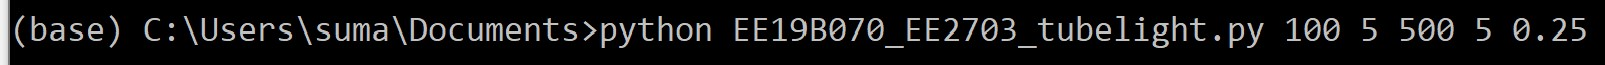
\includegraphics[scale = 1]{ss1.jpg}
    \caption{Visual representation of input}
\end{figure}

\subsubsection{Input Value Checks}
The first 3 inputs are required to be integers while the last 2 can be floats. The code checks whether this is True and will throw out an error if it is False. This is done with a try except loop.\\

We get the input values from the user using import sys library and using the sys.argv command.


\subsubsection{Code}
\begin{python}
if len(sys.argv) != 6:
	print("There has to be 6 integer inputs")

inp = sys.argv
input_int = ['']*(5)

#checks if first 3 inputs are integers
for n in range(3):
	try:
		input_int[n] = int(sys.argv[n+1])
	except ValueError:
	    print("Some of the first 3 inputs are NOT an integer, please check!!")
	    break
	else:
		input_int[n] = int(sys.argv[n+1])

#checks if last 2 inputs are floating integers
for n in range(2):
	try:
		input_int[n+3] = float(sys.argv[n+4])
	except ValueError:
	    print("Some of the last 2 inputs are NOT a rational number, please check!!")
	    break
	else:
		input_int[n+3] = float(sys.argv[n+4])
\end{python}

\subsection{Assigning the parameters}
\subsubsection{Code}
\begin{python}
#assigning the values

n = input_int[0]
M = input_int[1]
nk = input_int[2]
u0 = input_int[3]
p = input_int[4]
\end{python}

\subsection{Main code}
Our code mainly consists of a repeating for block with code inside it.\\The code is give below, analysis of the code is also below.
\begin{python}
#begin for loop
for i in range(1,nk): #iterate the block nk times
	ii = where(xx > 0)[0] 	#finds location of all existing electrons
	dx[ii] = u[ii] + 0.5	#gives us change in location
	xx[ii] = xx[ii] + dx[ii]	#adding this change
	u[ii] = u[ii] + 1			#change in velcity due to the constant acceleration

	out_of_bounds = where(xx > n)[0]	#finds location of all electrons out of bounds
	xx[out_of_bounds] = 0				#initialising all the values of these electrons to 0
	u[out_of_bounds] = 0
	dx[out_of_bounds] = 0

	#defing the deviation of electrons added per turn
	Msig = 2

	#for the collisions
	kk = where(u > u0)	#finds location of all electrons that can cause collisions
	ll=where(random.rand(len(kk[0]))<=p)[0];	#random distrinution of electrons that collide
	kl=kk[0][ll];								

	u[kl] = 0	#velocity of electrons after collision is 0
	xx[kl] = xx[kl] - dx[kl]*random.rand(len(kl))	#new electron position

	I.extend(xx[kl].tolist())	#adding all of these elctrons to our I vector
	m=int(random.rand()*Msig+M)	#number of electrons added is 5 with a standard deviation of 2

	empty = where(xx == 0)[0]
	tt = min(len(empty),m)		#checking which one is smaller

	xx[empty[:tt]] = 1	#setting the position of these elecrons to 1 and the rest of their values to 0
	u[empty[:tt]] = 0
	dx[empty[:tt]] = 0


	ii = where(xx > 0)[0]	#again we find existing electrons and add it to X and V
	X.extend(xx[ii].tolist())
	V.extend(u[ii].tolist())
\end{python}

\subsection{Analysing the code}
\subsubsection{The For loop}
loop is iterated nk times, so code is of the form:
\begin{verbatim}
    for k=1:nk
        <<block>>
    end
\end{verbatim}

\subsubsection{Initialising the vectors}
We initialise 3 vectors that we will use in our plots. These 3 vectors are:
\begin{verbatim}
     Intensity of emitted light, I
     Electron position, X
     Electron velocity, V
\end{verbatim}

\subsubsection{Finding existing electrons}
We find these electrons by using the where command. This would be:
\begin{verbatim}
    ii = where(xx > 0)
\end{verbatim}
this command would give us all the positions of existing electrons.

\subsubsection{Random Function}
the random function we used is
\begin{verbatim}
    random.rand(length)
\end{verbatim}
this code would give us a list of random numbers between 0 and 1 of given length.

\subsubsection{Number of electrons injected}
The number of electrons injected is not always 5, but rather it is a bell curve with maximum probability being 5 and with a standard deviation of 2. \\

This function is the reason why we get similar but different graphs every time.

\subsection{Plots}
We have 4 plots per given set of parameters. We mainly use the \textbf{\textit{hist}} command to plot them.

\subsubsection{Histogram plot of X vs x}
Here, X is the number of electrons.
\begin{python}
#plot the number of electrons vs x
hist(X, bins = arange(0,101), rwidth=0.75, color = 'purple')
title('Number of Electrons vs $x$ with $u_0=$%0.3f and p=%0.3f'%(u0,p))
xlabel('$x$')
ylabel('Number of electrons')
show()
\end{python}

\begin{figure}[H]
    \centering
    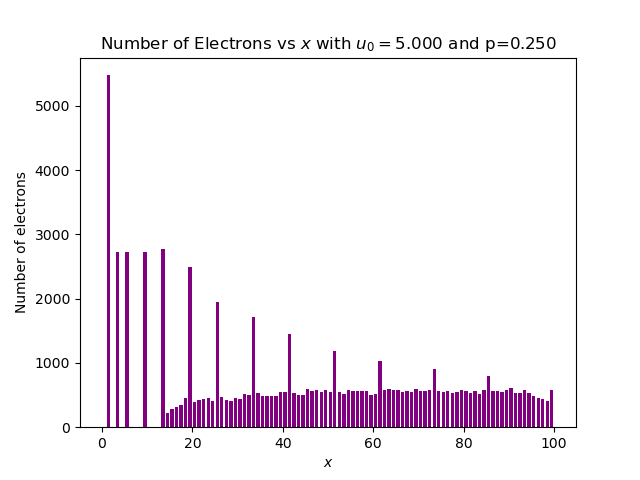
\includegraphics[scale = 1]{1_a.png}
    \caption{electron density vs position histogram plot for given values}
\end{figure}


\subsubsection{Histogram plot of I vs x}
Here, I is the Intensity.
\begin{python}
#plot the Intensity vs x
hist(I, bins = arange(0,101), rwidth=0.75, color = 'red')
title('Intensity vs $x$ with $u_0=$%0.3f and p=%0.3f'%(u0,p))
xlabel('$x$')
ylabel('Intensity')
show()
\end{python}

\begin{figure}[H]
    \centering
    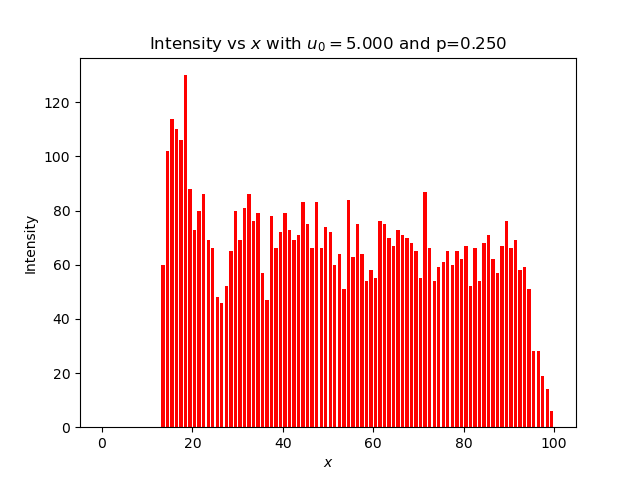
\includegraphics[scale = 1]{1_b.png}
    \caption{Intensity vs position histogram plot for given values}
\end{figure}

\subsubsection{Plot of V vs X}
Here, V is the velocity. X is the x-axis and V is the y-axis. We us a \textbf{x}, cross marker at each plot point.
\begin{python}
#electron phase plot
plot(X,V,'bx')
title('Electron phase plot with $u_0=$%0.3f and p=%0.3f'%(u0,p))
xlabel('$x$')
ylabel('$v$')
show()
\end{python}

\begin{figure}[H]
    \centering
    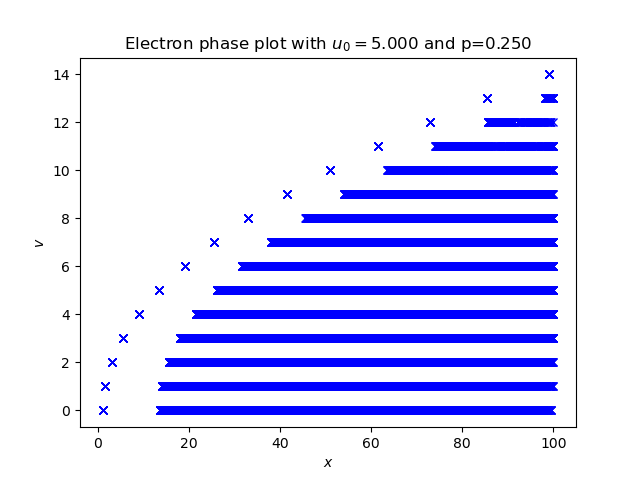
\includegraphics[scale = 1]{1_c.png}
    \caption{electron density vs velocity plot}
\end{figure}

\subsubsection{Intensity density plot}

This plot is amazing, as it basically shows us how the real life light bulb would would look like. We have used the $Greys_r$ colormap that indicates the bright and dark regions of the tubelight.

\begin{python}
#plots the Intensity density plot
bins = arange(0,101)
hist, edges = np.histogram(I, bins)
hist=hist[newaxis,:]
extent=[bins.min(), bins.max(),0,1]
imshow(hist, aspect = "auto", cmap="Greys_r", extent=extent)
title('Intensity Density plot with $u_0=$%0.3f and p=%0.3f'%(u0,p))
gca().set_yticks([])
colorbar()
show()

\end{python}

\begin{figure}[H]
    \centering
    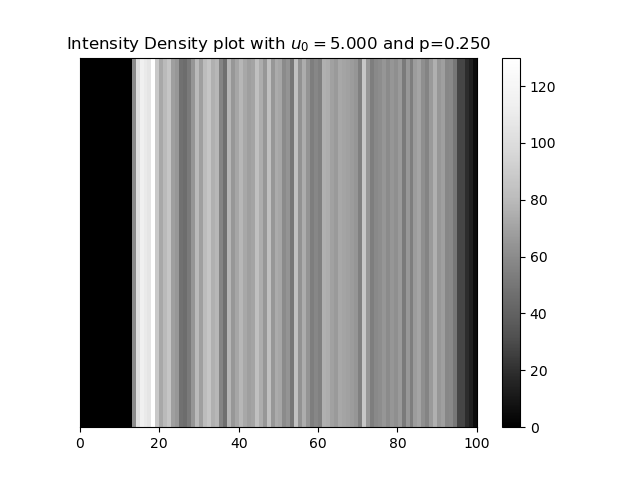
\includegraphics[scale = 1]{1_d.png}
    \caption{Intensity density plot}
\end{figure}




\subsection{Answering Assignment Questions}
\subsubsection{Question1}
Yes, we can actually get a better estimation for apparent dx using a \textbf{Random TIME} instead of a random number multiplied by dx.
we then find this random time and find
\begin{equation}
    dx'[kl] = u[kl]*tt + 0.5*(tt)^2
\end{equation}

\subsubsection{Question2}
Yes, we can use the last ii as the initial ii of the next iteration.\\

To do this we, would need to define one loop of the for loop as a function that also returns the set ii as an outut. We can define this set ii as an input of the function as well. So now, the output ii is used as the input ii for the next loop.

\subsubsection{Question3}
We see that we get more priminent black spaces when we increase u0 (thresh hold velocity) and decrease p (probability that ionization will occur).\\

We can see a prominent dark region for u0 = 7 and p = 0.25. (For visualisation, see the intensity density plot below).

\subsection{Remaining Plots}

\subsubsection{For u0 = 5 and p = 0.5}

\begin{figure}[H]
    \centering
    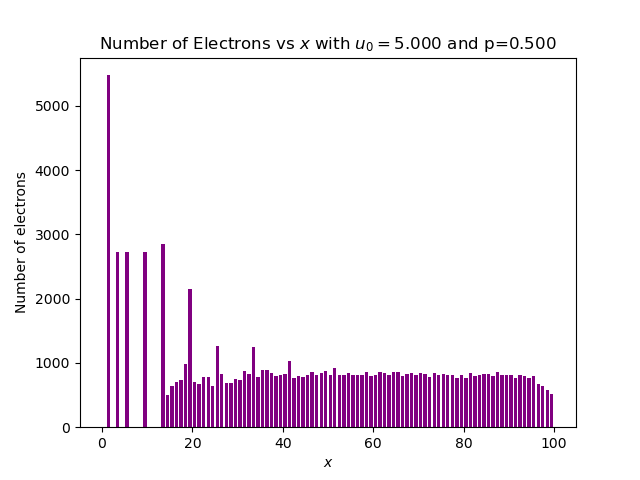
\includegraphics[scale = 1]{2_a.png}
    \caption{electron density vs position histogram plot for given values}
\end{figure}

\begin{figure}[H]
    \centering
    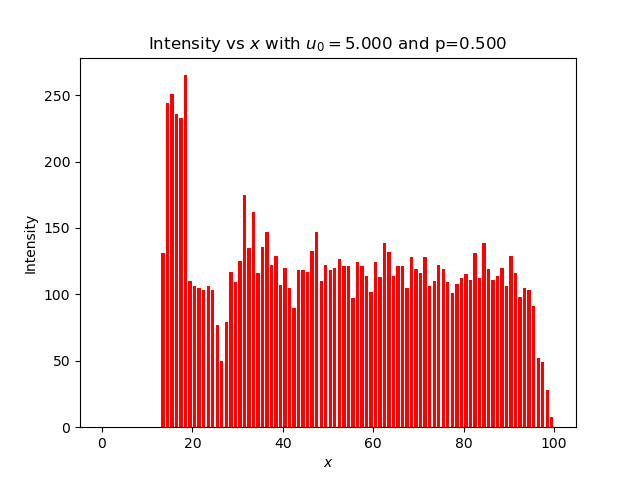
\includegraphics[scale = 1]{2_b.png}
    \caption{Intensity vs position histogram plot for given values}
\end{figure}

\begin{figure}[H]
    \centering
    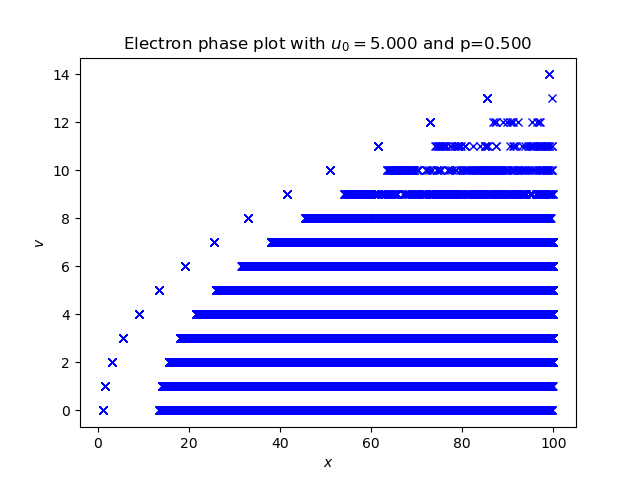
\includegraphics[scale = 1]{2_c.png}
    \caption{electron density vs velocity plot}
\end{figure}

\begin{figure}[H]
    \centering
    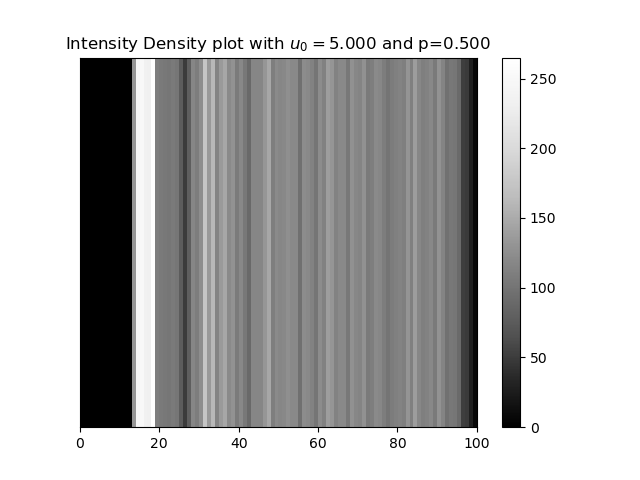
\includegraphics[scale = 1]{2_d.png}
    \caption{Intensity density plot}
\end{figure}

\subsubsection{For u0 = 7 and p = 0.5}

\begin{figure}[H]
    \centering
    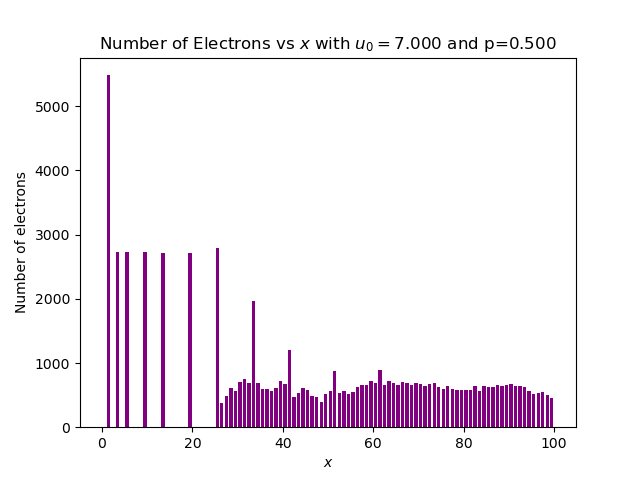
\includegraphics[scale = 1]{3_a.png}
    \caption{electron density vs position histogram plot for given values}
\end{figure}

\begin{figure}[H]
    \centering
    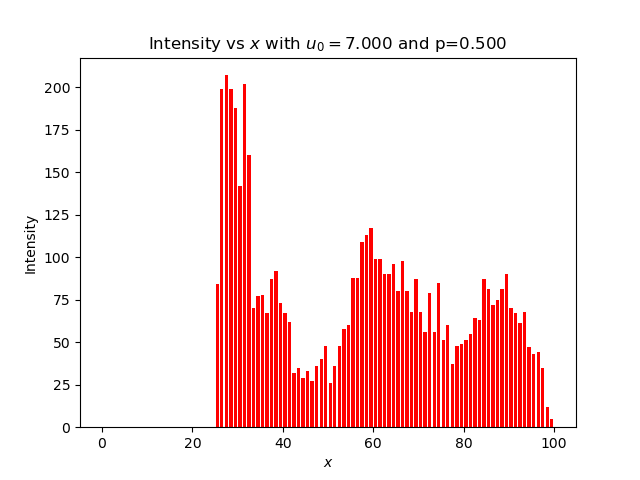
\includegraphics[scale = 1]{3_b.png}
    \caption{Intensity vs position histogram plot for given values}
\end{figure}

\begin{figure}[H]
    \centering
    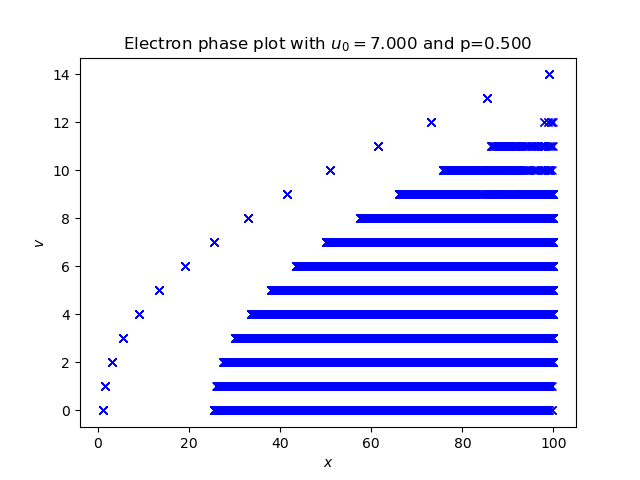
\includegraphics[scale = 1]{3_c.png}
    \caption{electron density vs velocity plot}
\end{figure}

\begin{figure}[H]
    \centering
    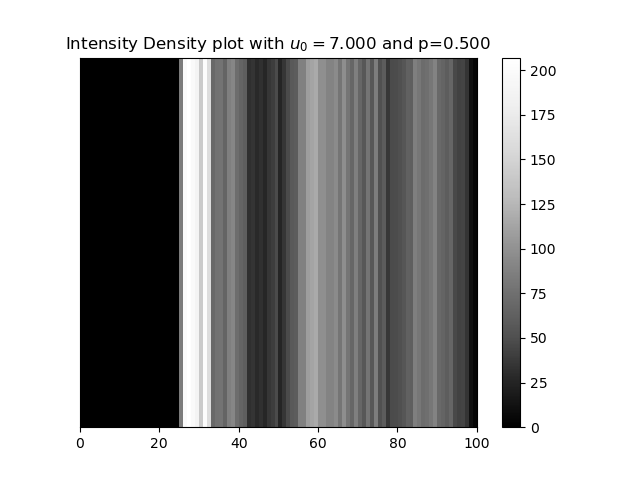
\includegraphics[scale = 1]{3_d.png}
    \caption{Intensity density plot}
\end{figure}

\subsubsection{For u0 = 2 and p = 0.75}

\begin{figure}[H]
    \centering
    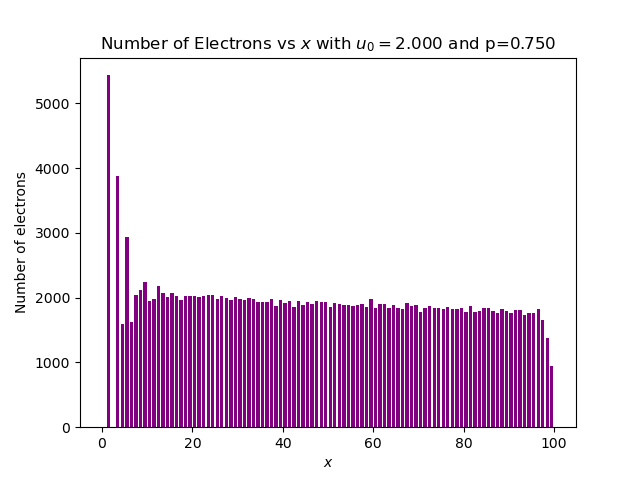
\includegraphics[scale = 1]{4_a.png}
    \caption{electron density vs position histogram plot for given values}
\end{figure}

\begin{figure}[H]
    \centering
    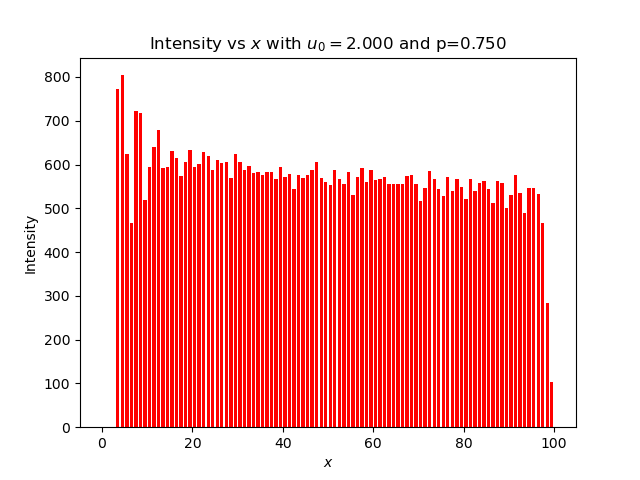
\includegraphics[scale = 1]{4_b.png}
    \caption{Intensity vs position histogram plot for given values}
\end{figure}

\begin{figure}[H]
    \centering
    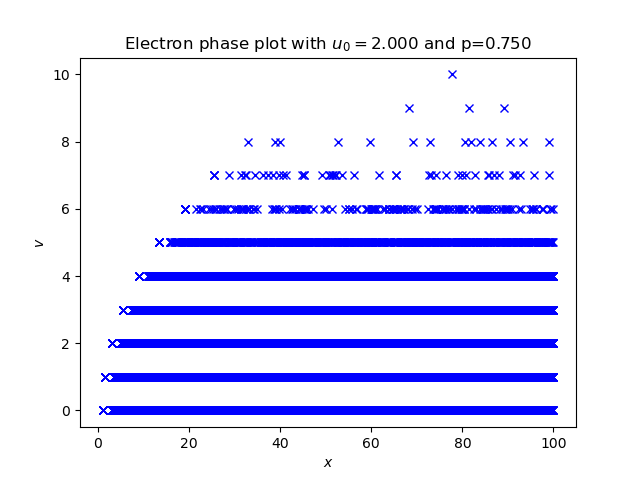
\includegraphics[scale = 1]{4_c.png}
    \caption{electron density vs velocity plot}
\end{figure}

\begin{figure}[H]
    \centering
    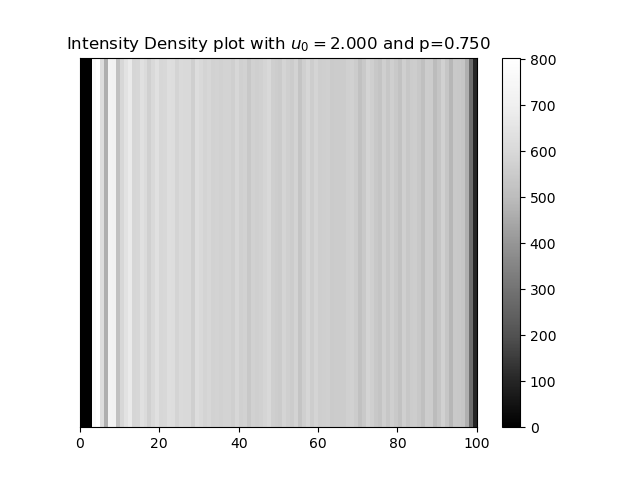
\includegraphics[scale = 1]{4_d.png}
    \caption{Intensity density plot}
\end{figure}








\end{document}